\documentclass[11pt,a4paper]{article}
\usepackage[margin=2.2cm]{geometry}
\usepackage{amsmath,amssymb}
\usepackage{booktabs}
\usepackage{enumitem}
\usepackage{hyperref}
\usepackage{xcolor}
\usepackage{tikz}
\usetikzlibrary{arrows.meta,positioning,calc}

\title{Social Dynamics Simulator:\\Mathematical Overview}
\author{}
\date{}

\begin{document}
\maketitle
\tableofcontents
\newpage

%% ================================================================
\section{Notation}

\begin{tabular}{ll}
\toprule
\textbf{Symbol} & \textbf{Definition} \\
\midrule
$N$ & Number of particles \\
$K$ & Number of preference dimensions per particle \\
$i, j$ & Particle indices, $i, j \in \{1, \ldots, N\}$ \\
$d$ & Preference dimension index, $d \in \{1, \ldots, K\}$ \\
$\mathbf{x}_i \in [0, L)^2$ & Position of particle $i$ (toroidal domain, $L = 1$) \\
$\mathbf{p}_i \in [-1, 1]^K$ & Signal (preference) vector of particle $i$ \\
$\mathbf{r}_i \in [-1, 1]^K$ & Response vector of particle $i$ \\
$\mathcal{N}(i)$ & Neighbor set of particle $i$ \\
$j^*_d(i)$ & Best neighbor of $i$ in dimension $d$ \\
$\eta$ & Step size \\
$L$ & Domain size (default 1.0, toroidal) \\
$\Delta(\mathbf{a}, \mathbf{b})$ & Periodic displacement: $\mathbf{b} - \mathbf{a} - L \cdot \mathrm{round}\!\left(\frac{\mathbf{b} - \mathbf{a}}{L}\right)$ \\
\bottomrule
\end{tabular}

%% ================================================================
\section{Core Dynamics: Per-Dimension Max-Preference Physics}

The fundamental interaction rule: each particle moves toward the neighbors that have the strongest preference values, weighted by its own preferences.

\subsection{Algorithm}

For each particle $i$ at each time step:

\begin{enumerate}[nosep]
\item \textbf{Find neighbors}: Determine $\mathcal{N}(i)$, the set of nearby particles (via KNN or radius search).

\item \textbf{Per-dimension best neighbor}: For each dimension $d \in \{1, \ldots, K\}$, find the neighbor with the highest signal value:
\begin{equation}
j^*_d(i) = \arg\max_{j \in \mathcal{N}(i)} \; p_j^{(d)}
\end{equation}

\item \textbf{Direction}: Compute the unit direction from $i$ toward each best neighbor (periodic):
\begin{equation}
\hat{\mathbf{u}}_d(i) = \frac{\Delta(\mathbf{x}_i,\, \mathbf{x}_{j^*_d})}{\|\Delta(\mathbf{x}_i,\, \mathbf{x}_{j^*_d})\|}
\end{equation}

\item \textbf{Compatibility}: The weight for dimension $d$ is the product of the particle's own response and the best neighbor's signal:
\begin{equation}
w_d(i) = r_i^{(d)} \cdot p_{j^*_d}^{(d)}
\end{equation}

\item \textbf{Movement}: Sum the weighted directions across all dimensions:
\begin{equation}
\mathbf{v}_i = \sum_{d=1}^{K} w_d(i) \cdot \hat{\mathbf{u}}_d(i)
\end{equation}

\item \textbf{Position update}:
\begin{equation}
\mathbf{x}_i \leftarrow \left(\mathbf{x}_i + \eta \cdot \mathbf{v}_i\right) \bmod L
\end{equation}
\end{enumerate}

\subsection{Worked Example: 3 Particles, $K = 3$}

Consider three particles $A$, $B$, $C$ with positions and preferences:

\begin{center}
\begin{tabular}{cccc}
\toprule
Particle & Position & Signal $\mathbf{p}$ & Response $\mathbf{r}$ \\
\midrule
$A$ & $(0.3, 0.5)$ & $(0.8, -0.3, 0.5)$ & $(0.8, -0.3, 0.5)$ \\
$B$ & $(0.6, 0.4)$ & $(0.2, 0.9, -0.7)$ & $(0.2, 0.9, -0.7)$ \\
$C$ & $(0.5, 0.8)$ & $(-0.4, 0.6, 0.9)$ & $(-0.4, 0.6, 0.9)$ \\
\bottomrule
\end{tabular}
\end{center}

Without signal/response split, $\mathbf{r}_i = \mathbf{p}_i$.

\vspace{0.5em}
\textbf{Step 1}: All particles are neighbors of each other ($N = 3$, $K_{\mathrm{nn}} = 2$).

\textbf{Step 2}: For particle $A$, find the best neighbor per dimension:

\begin{center}
\begin{tabular}{clcl}
\toprule
Dim $d$ & Best neighbor & $p_{j^*}^{(d)}$ & Why \\
\midrule
1 & $B$ ($p^{(1)} = 0.2$) & 0.2 & $\max(0.2, -0.4) = 0.2$ \\
2 & $B$ ($p^{(2)} = 0.9$) & 0.9 & $\max(0.9, 0.6) = 0.9$ \\
3 & $C$ ($p^{(3)} = 0.9$) & 0.9 & $\max(-0.7, 0.9) = 0.9$ \\
\bottomrule
\end{tabular}
\end{center}

\textbf{Step 3}: Directions from $A$ toward each best neighbor:
\begin{align*}
\hat{\mathbf{u}}_1 &= \hat{\mathbf{u}}_2 = \mathrm{normalize}(B - A) = \mathrm{normalize}(0.3, -0.1) \approx (0.949, -0.316) \\
\hat{\mathbf{u}}_3 &= \mathrm{normalize}(C - A) = \mathrm{normalize}(0.2, 0.3) \approx (0.555, 0.832)
\end{align*}

\textbf{Step 4}: Compatibility weights (response $\times$ signal):
\begin{align*}
w_1 &= r_A^{(1)} \cdot p_B^{(1)} = 0.8 \times 0.2 = 0.16 \\
w_2 &= r_A^{(2)} \cdot p_B^{(2)} = -0.3 \times 0.9 = -0.27 \\
w_3 &= r_A^{(3)} \cdot p_C^{(3)} = 0.5 \times 0.9 = 0.45
\end{align*}

Note: $w_2 < 0$ means particle $A$ moves \emph{away} from $B$ on dimension 2 (opposite preferences).

\textbf{Step 5}: Total movement:
\begin{align*}
\mathbf{v}_A &= 0.16 \cdot (0.949, -0.316) + (-0.27) \cdot (0.949, -0.316) + 0.45 \cdot (0.555, 0.832) \\
&= (0.152, -0.051) + (-0.256, 0.085) + (0.250, 0.374) \\
&= (0.146, 0.409)
\end{align*}

\begin{center}
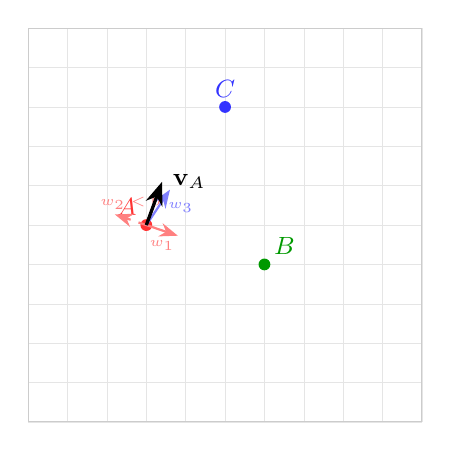
\begin{tikzpicture}[scale=5, >=Stealth]
  % Grid
  \draw[gray!20, very thin] (0,0) grid[step=0.1] (1,1);
  \draw[gray!40, thin] (0,0) rectangle (1,1);

  % Particles
  \fill[red!80] (0.3, 0.5) circle (0.015) node[above left, font=\small] {$A$};
  \fill[green!60!black] (0.6, 0.4) circle (0.015) node[above right, font=\small] {$B$};
  \fill[blue!80] (0.5, 0.8) circle (0.015) node[above, font=\small] {$C$};

  % Direction arrows from A
  \draw[->, red!50, thick] (0.3, 0.5) -- ++(0.08, -0.027) node[midway, below, font=\tiny] {$w_1$};
  \draw[->, red!50, dashed, thick] (0.3, 0.5) -- ++(-0.08, 0.027) node[midway, above, font=\tiny] {$w_2<0$};
  \draw[->, blue!50, thick] (0.3, 0.5) -- ++(0.06, 0.09) node[midway, right, font=\tiny] {$w_3$};

  % Resultant
  \draw[->, black, very thick] (0.3, 0.5) -- ++(0.04, 0.11) node[right, font=\small] {$\mathbf{v}_A$};
\end{tikzpicture}
\end{center}

\textbf{Key insight}: Dimensions 1 and 2 both point toward $B$, but with opposite signs. Dimension 3 points toward $C$. The resultant movement depends on the \emph{balance} of these competing forces.

%% ================================================================
\section{Best Neighbor Selection Modes}

The selection of $j^*_d(i)$ can be modified:

\subsection{Mode 0: Default (highest value)}
\begin{equation}
j^*_d(i) = \arg\max_{j \in \mathcal{N}(i)} \; p_j^{(d)}
\end{equation}
Selects the neighbor with the highest raw preference. Positive values are preferred over negative.

\subsection{Mode 1: Max Magnitude}
\begin{equation}
j^*_d(i) = \arg\max_{j \in \mathcal{N}(i)} \; |p_j^{(d)}|
\end{equation}
Selects the neighbor with the strongest preference regardless of sign.

\subsection{Mode 2: Same-Sign Max Magnitude}
\begin{equation}
j^*_d(i) = \arg\max_{\substack{j \in \mathcal{N}(i) \\ \mathrm{sign}(p_j^{(d)}) = \mathrm{sign}(p_i^{(d)})}} \; |p_j^{(d)}|
\end{equation}
Only considers neighbors whose preference has the same sign as particle $i$ in dimension $d$. If no same-sign neighbor exists, dimension $d$ contributes zero to the movement.

%% ================================================================
\section{Inner-Product Average Mode}

An alternative to the per-dimension best-neighbor selection. Instead of finding one best neighbor per dimension, this mode weights \emph{all} neighbors by the full inner product of their preference vectors:

\begin{equation}
\mathbf{v}_i = \frac{1}{|\mathcal{N}(i)|} \sum_{j \in \mathcal{N}(i)} \frac{\mathbf{r}_i \cdot \mathbf{p}_j}{K} \cdot \hat{\mathbf{u}}_{ij}
\end{equation}

where $\hat{\mathbf{u}}_{ij} = \Delta(\mathbf{x}_i, \mathbf{x}_j) / \|\Delta(\mathbf{x}_i, \mathbf{x}_j)\|$.

Particles with aligned preferences attract ($\mathbf{r}_i \cdot \mathbf{p}_j > 0$), while misaligned particles repel.

%% ================================================================
\section{Signal / Response Split}

By default, $\mathbf{r}_i = \mathbf{p}_i$. The signal/response split separates these into independent vectors:

\begin{itemize}[nosep]
\item \textbf{Signal} $\mathbf{p}_i$: what particle $i$ broadcasts. Used by other particles for neighbor selection ($\arg\max p_j^{(d)}$).
\item \textbf{Response} $\mathbf{r}_i$: how particle $i$ reacts. Used in the compatibility weight ($w_d = r_i^{(d)} \cdot p_{j^*}^{(d)}$).
\end{itemize}

This breaks the symmetry: a particle can listen for signals it doesn't broadcast, or broadcast signals it doesn't respond to.

\subsection{Compatibility}

With the split:
\begin{equation}
w_d(i) = r_i^{(d)} \cdot p_{j^*_d}^{(d)}
\end{equation}

The selection $j^*_d$ always uses the \textbf{signal} vector of the neighbors. The weighting uses the \textbf{response} of particle $i$ and the \textbf{signal} of the selected neighbor.

%% ================================================================
\section{Repulsion}

An optional repulsive force pushes particles away from close neighbors:

\begin{equation}
\mathbf{v}_i^{\mathrm{rep}} = -\frac{\rho}{|\mathcal{N}(i)|} \sum_{j \in \mathcal{N}(i)} \frac{\hat{\mathbf{u}}_{ij}}{\|\Delta(\mathbf{x}_i, \mathbf{x}_j)\|}
\end{equation}

where $\rho$ is the repulsion strength. The $1/r$ scaling creates stronger repulsion at close range.

%% ================================================================
\section{Social Learning}

Preferences evolve over time via social learning from neighbors:

\begin{equation}
\mathbf{p}_i \leftarrow (1 - s) \cdot \mathbf{p}_i + s \cdot \bar{\mathbf{p}}_{\mathcal{N}(i)}
\end{equation}

where $\bar{\mathbf{p}}_{\mathcal{N}(i)} = \frac{1}{|\mathcal{N}(i)|} \sum_{j \in \mathcal{N}(i)} \mathbf{p}_j$ is the neighbor mean preference.

\begin{itemize}[nosep]
\item $s > 0$: \textbf{Conformity} --- preferences move toward the local mean.
\item $s < 0$: \textbf{Differentiation} --- preferences move away from the local mean.
\item $s = 0$: Preferences are fixed.
\end{itemize}

\subsection{Quiet-Dimension Differentiation}

Instead of uniform social learning across all dimensions, scale the learning rate inversely by each dimension's contribution to movement:

\begin{equation}
s_d(i) = s \cdot \left(1 - \frac{|w_d(i)|}{\max_{d'} |w_{d'}(i)|}\right)
\end{equation}

Dimensions that contribute most to movement (high $|w_d|$) are preserved. Dimensions that contribute least (low $|w_d|$) are differentiated most. This allows particles to specialize on ``quiet'' dimensions without disrupting the primary dynamics.

%% ================================================================
\section{Spatial Memory Field}

A persistent grid field $M \in \mathbb{R}^{G \times G \times K}$ creates feedback between dynamics and environment.

\subsection{Read (before physics)}
\begin{equation}
\tilde{p}_i^{(d)} = p_i^{(d)} \cdot \left(1 + \alpha \cdot M\!\left(\mathrm{cell}(\mathbf{x}_i), d\right)\right)
\end{equation}
Clipped to $[-1, 1]$. The field amplifies aligned preferences and dampens opposed ones.

\subsection{Write (after physics)}
\begin{equation}
M\!\left(\mathrm{cell}(\mathbf{x}_i), d\right) \mathrel{+}= \beta \cdot p_i^{(d)}
\end{equation}

\subsection{Decay}
\begin{equation}
M \leftarrow \gamma \cdot M
\end{equation}

\subsection{Blur (optional)}
\begin{equation}
M^{(d)} \leftarrow M^{(d)} * \mathcal{G}(\sigma)
\end{equation}
Gaussian diffusion with periodic wrapping.

See \texttt{spatial\_memory.pdf} for detailed analysis of regimes and fixed points.

%% ================================================================
\section{Neighbor Finding}

\subsection{KNN (K-Nearest Neighbors)}
Find the $K_{\mathrm{nn}}$ closest particles by periodic Euclidean distance. Implemented via:
\begin{itemize}[nosep]
\item \textbf{cKDTree}: $O(N \log N)$ build, $O(K_{\mathrm{nn}} \log N)$ per query. Best for KNN.
\item \textbf{Spatial Hash Grid}: $O(N)$ build, ring-expansion query. Best for radius queries.
\end{itemize}

\subsection{Radius}
Find all particles within distance $R$. Neighbor count varies per particle (can be very large in clusters).

\subsection{KNN + Radius}
Find $K_{\mathrm{nn}}$ nearest, then filter to those within radius $R$. Bounded cost with distance cutoff.

%% ================================================================
\section{Grid Field Approximations}

For large $N$, pairwise neighbor search becomes the bottleneck. Grid-based methods approximate the physics at $O(N + G^2)$ cost.

\subsection{Smooth Grid Field}

Deposit preferences onto a $G \times G$ grid via bilinear interpolation, Gaussian-smooth, compute gradients:

\begin{equation}
\mathbf{v}_i = \sum_{d=1}^{K} r_i^{(d)} \cdot \nabla F^{(d)}(\mathbf{x}_i)
\end{equation}

where $F^{(d)}$ is the smoothed signal field for dimension $d$.

\subsection{Grid Max Field}

Approximates the per-dimension best-neighbor physics on a grid:

\begin{enumerate}[nosep]
\item \textbf{Deposit}: For each cell, store the max signal value per dim and the source particle's position.
\item \textbf{Propagate}: Iterative 3$\times$3 max-pool (8-connected) spreads max values to neighboring cells, carrying source positions. After $P$ passes, each cell knows the best particle within Chebyshev distance $P$.
\item \textbf{Movement}: Each particle reads its cell's per-dim max and source position:
\begin{equation}
\mathbf{v}_i = \sum_{d=1}^{K} r_i^{(d)} \cdot M_d^{\max}(\mathrm{cell}(\mathbf{x}_i)) \cdot \hat{\mathbf{u}}_d^{\max}(\mathrm{cell}(\mathbf{x}_i))
\end{equation}
\end{enumerate}

The GPU variant uses fused \texttt{max\_pool2d} with \texttt{return\_indices} for single-kernel propagation.

%% ================================================================
\section{Force Landscape}

The force landscape answers: ``at each point in space, what preference vector would produce the maximum movement?''

For a probe at position $\mathbf{x}$, the movement is linear in the response vector:
\begin{equation}
\mathbf{v}(\mathbf{x}, \mathbf{r}) = \mathbf{M}(\mathbf{x}) \cdot \mathbf{r}
\end{equation}

where $\mathbf{M}(\mathbf{x})$ is the $2 \times K$ matrix with columns $p_{j^*_d}^{(d)} \cdot \hat{\mathbf{u}}_d$, built from the actual KNN neighbors at position $\mathbf{x}$.

The optimal response is found by exhaustive search over $\{-1, 0, +1\}^K$ ($3^K$ candidates):
\begin{equation}
\mathbf{r}^* = \arg\max_{\mathbf{r} \in \{-1,0,+1\}^K} \|\mathbf{M}(\mathbf{x}) \cdot \mathbf{r}\|
\end{equation}

Three visualization modes:
\begin{itemize}[nosep]
\item \textbf{Max Pref}: the per-dim max signal values as RGB, brightness by force magnitude.
\item \textbf{Optimal Pref}: the optimal $\mathbf{r}^*$ as RGB.
\item \textbf{Direction}: angle of $\mathbf{M} \cdot \mathbf{r}^*$ as HSV hue, magnitude as brightness.
\end{itemize}

An exponential moving variance mode shows temporal stability:
\begin{align}
\mu_t &= \gamma \mu_{t-1} + (1 - \gamma) x_t \\
\sigma^2_t &= \gamma \left(\sigma^2_{t-1} + (1 - \gamma)(x_t - \mu_{t-1})^2\right)
\end{align}

%% ================================================================
\section{Shadow Simulation}

A deep copy of the simulation with LSB-perturbed positions tracks chaotic sensitivity:

\begin{equation}
\tilde{\mathbf{x}}_i = \mathbf{x}_i \oplus \delta_i
\end{equation}

where $\delta_i$ randomizes the lowest $B$ bits of the IEEE 754 mantissa. For $B = 1$, the perturbation is $\sim 10^{-16}$ (one ULP).

Divergence is measured as RMS periodic distance:
\begin{equation}
D(t) = \sqrt{\frac{1}{N} \sum_{i=1}^{N} \|\Delta(\mathbf{x}_i(t),\, \tilde{\mathbf{x}}_i(t))\|^2}
\end{equation}

Exponential growth of $D(t)$ indicates chaotic dynamics.

%% ================================================================
\section{Precision Controls}

\subsection{Dtype Selection}
\begin{itemize}[nosep]
\item Positions: \texttt{float32} or \texttt{float64}
\item Preferences: \texttt{float16} (10-bit mantissa), \texttt{float32} (23-bit), or \texttt{float64} (52-bit)
\item Physics compute (PyTorch): \texttt{float16}, \texttt{bfloat16}, \texttt{float32}, \texttt{float64}
\end{itemize}

\subsection{Mantissa Truncation}

After each step, zero the lowest $(M - B)$ mantissa bits:
\begin{equation}
x_{\mathrm{trunc}} = \mathrm{int}(x) \gg (M - B) \ll (M - B)
\end{equation}
where $M$ is the full mantissa width and $B$ is the target bits.

\subsection{Level Quantization}

Snap preferences to $Q$ evenly spaced values in $[-1, 1]$:
\begin{equation}
p_{\mathrm{quant}} = \frac{\mathrm{round}\!\left(\frac{p + 1}{2} \cdot (Q - 1)\right)}{Q - 1} \cdot 2 - 1
\end{equation}

Special case $Q = 2$: binary $\{-1, +1\}$ via $\mathrm{sign}(p)$.

%% ================================================================
\section{Direction Memory}

An exponential moving average (EMA) of the per-dimension direction vectors:
\begin{equation}
\mathbf{d}_i^{(k)} \leftarrow \lambda \cdot \mathbf{d}_i^{(k)} + (1 - \lambda) \cdot \hat{\mathbf{u}}_k(i)
\end{equation}

where $\lambda$ is the direction memory parameter. The movement then uses $\mathbf{d}_i^{(k)}$ instead of $\hat{\mathbf{u}}_k(i)$, giving particles momentum that persists across neighbor changes.

%% ================================================================
\section{Full Update Rule}

Combining all components, the complete per-step update for particle $i$ is:

\begin{enumerate}[nosep]
\item Read memory field: $\tilde{\mathbf{p}}_i = \mathbf{p}_i \cdot (1 + \alpha \cdot M(\mathrm{cell}(\mathbf{x}_i)))$
\item Find neighbors $\mathcal{N}(i)$
\item For each dim $d$: find $j^*_d$, compute $\hat{\mathbf{u}}_d$, update direction memory $\mathbf{d}_d$
\item Compute compatibility: $w_d = \tilde{r}_i^{(d)} \cdot \tilde{p}_{j^*_d}^{(d)}$
\item Optionally multiply by inner product: $w_d \mathrel{\times}= \frac{\tilde{\mathbf{r}}_i \cdot \tilde{\mathbf{p}}_{j^*_d}}{K}$
\item Movement: $\mathbf{v}_i = \sum_d w_d \cdot \mathbf{d}_d + \mathbf{v}_i^{\mathrm{rep}}$
\item Update position: $\mathbf{x}_i \leftarrow (\mathbf{x}_i + \eta \cdot \mathbf{v}_i) \bmod L$
\item Social learning: $\mathbf{p}_i \leftarrow (1 - s_d) \cdot \mathbf{p}_i + s_d \cdot \bar{\mathbf{p}}_{\mathcal{N}(i)}$
\item Write memory field: $M(\mathrm{cell}(\mathbf{x}_i)) \mathrel{+}= \beta \cdot \mathbf{p}_i$
\item Decay memory: $M \leftarrow \gamma \cdot M$; optionally blur $M$
\item Optionally truncate/quantize $\mathbf{x}_i$ and $\mathbf{p}_i$
\end{enumerate}

\end{document}
